\documentclass[a4paper, 12pt]{amsart}
\usepackage[T1]{fontenc}
\usepackage{graphicx}
\usepackage{wrapfig}
\usepackage{tikz}
\usetikzlibrary{shapes.geometric}
\tikzset{
  half circle/.style={
      semicircle,
      shape border rotate=180,
      anchor=chord center,
      minimum size=5mm
      }
}
\author{PS}
\begin{document}
\section{Includegraphics}
Lorem ipsum dolor sit amet, consectetur adipiscing elit. Duis ut ex laoreet, bibendum est at, varius lorem. Duis sed purus nulla. Maecenas nec mauris sed erat mattis sagittis.
\begin{center}
\includegraphics[scale=2]{Kardioida.png}
\end{center}
\par Pellentesque a quam vulputate, scelerisque nulla a, suscipit elit. Suspendisse a posuere nunc. Duis commodo, justo eu tempor luctus, orci nisi rutrum elit, ac facilisis purus turpis id turpis. Curabitur sed arcu ullamcorper, gravida risus a, efficitur urna.
\newpage
\section{Wrapfigure}
Suspendisse urna mi, porta sit amet tristique id, interdum vitae ex. In in lectus et ipsum luctus tincidunt nec sed dui.
\begin{wrapfigure}{c}{0.30\textwidth}
\includegraphics[height=30ex, width=10em ]{stich.jpg}
\end{wrapfigure}
Proin a odio maximus, faucibus dolor et, tempor tortor. Aliquam finibus elementum ligula eu varius. Pellentesque eget ex aliquam, scelerisque sapien ac, porta ante. Donec maximus nibh velit, sit amet elementum dui consequat ac. Suspendisse ornare id orci ac imperdiet. Aliquam volutpat nunc vitae sapien aliquet rutrum. Praesent nec odio sed sem hendrerit fermentum. Duis fringilla tortor purus, a viverra orci lobortis vel. Praesent in lorem eu elit tempor rhoncus at ac erat. Nam dui nulla, fringilla vel pretium vitae, fringilla vulputate massa.
\section{Tikz}
\begin{tikzpicture}
\draw [blue, thick, ->, dashed] (-2,0) to (2,0);
\end{tikzpicture}

\begin{figure}[ht]
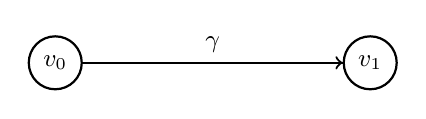
\begin{tikzpicture}[auto, node distance=4cm,
thick,main node/.style={circle,draw,font=\small\bfseries}]
\node[main node] (0) {$v_0$};
\node[main node] (1) [right of=0] {$v_1$};
\path[every node/.style={font=\small}]
(0) edge node [bend right] {$\gamma$} (1);
\draw[->] (0) to (1);
\end{tikzpicture}
\end{figure}

\begin{figure}[ht]
\centering
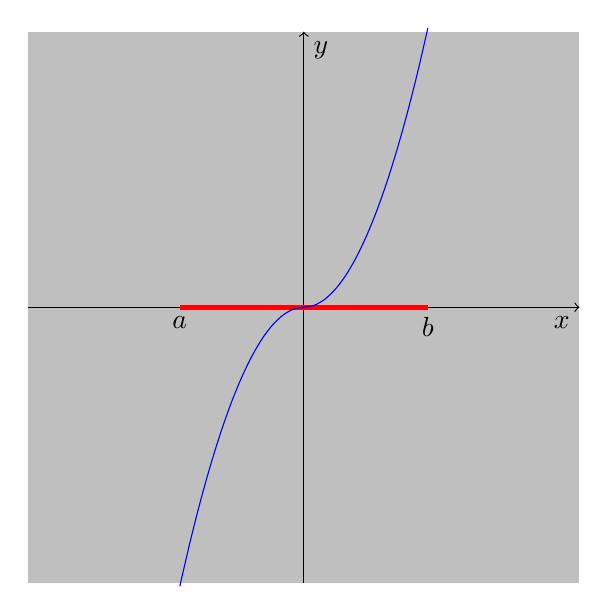
\begin{tikzpicture}[scale=0.7]
\path [draw=none,fill=gray,semitransparent] (-5,-5) rectangle (5,5);
\draw [->] (-5,0) to (5,0) node [below left] {$x$};
\draw [->] (0,-5) to (0,5) node [below right] {$y$};
\draw[red, line width = 0.70mm] (-2.25,0) to (2.25,0);
\node [below,black] at (2.25,0) {$b$};
\node [below ,black] at (-2.25,0) {$a$};
\draw[scale=1, domain=-2.25:2.25, smooth, variable=\x, blue] plot ({\x},{\x^2});
\end{tikzpicture}
\caption{$y=x^2$ na $(-2.25, 2.25)$}
\end{figure}

\begin{figure}[ht]
\centering
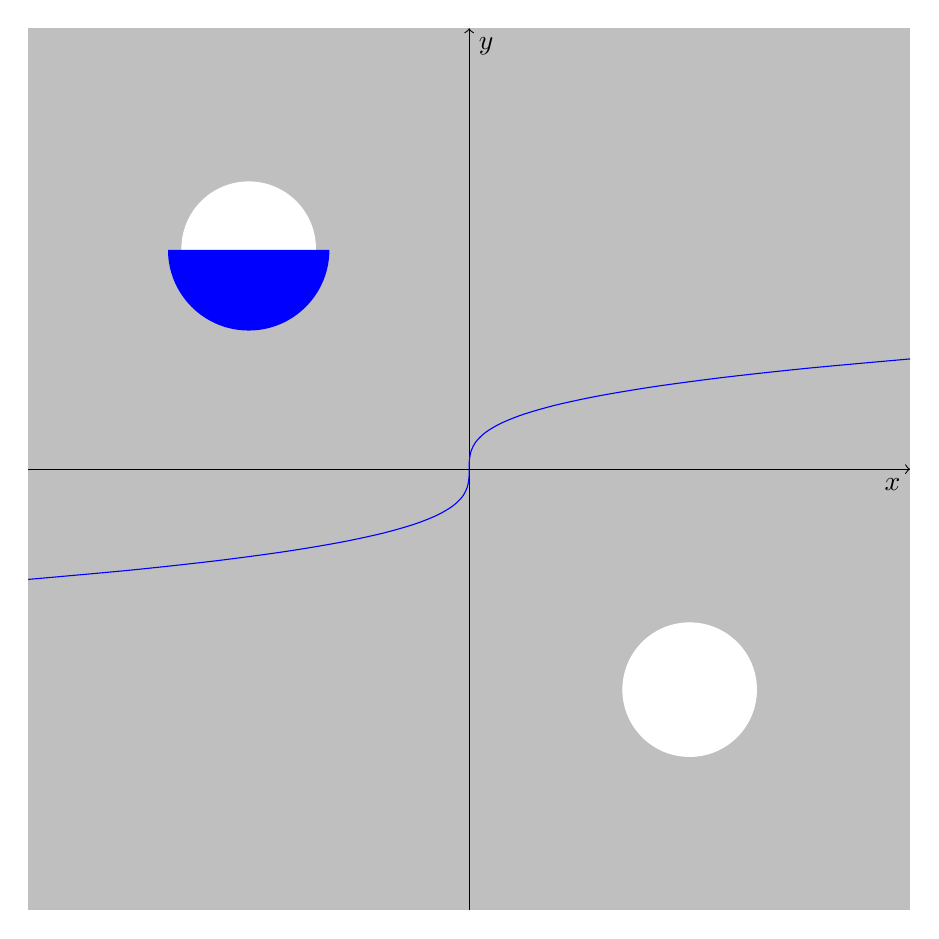
\begin{tikzpicture}[scale=0.7]
\path [draw=none,fill=gray,semitransparent] (-8,-8) rectangle (8,8);
\draw [->] (-8,0) to (8,0) node [below left] {$x$};
\draw [->] (0,-8) to (0,8) node [below right] {$y$};
\draw[white, fill=white] (-4,4) circle (8ex);
\node [half circle, white, fill=blue, scale=2.05] at (-4,4) {};
\draw[fill=white,white] (4,-4) circle (8ex);
\draw[scale=1, domain=-2:2, smooth, variable=\y, blue] plot ({\y^3},{\y});
\end{tikzpicture}
\caption{$y=\sqrt[3]{x}$ na $(-8, 8)$ oraz dwa koła}
\end{figure}
\newpage
\section{Domek}
\begin{figure}[ht]
\centering
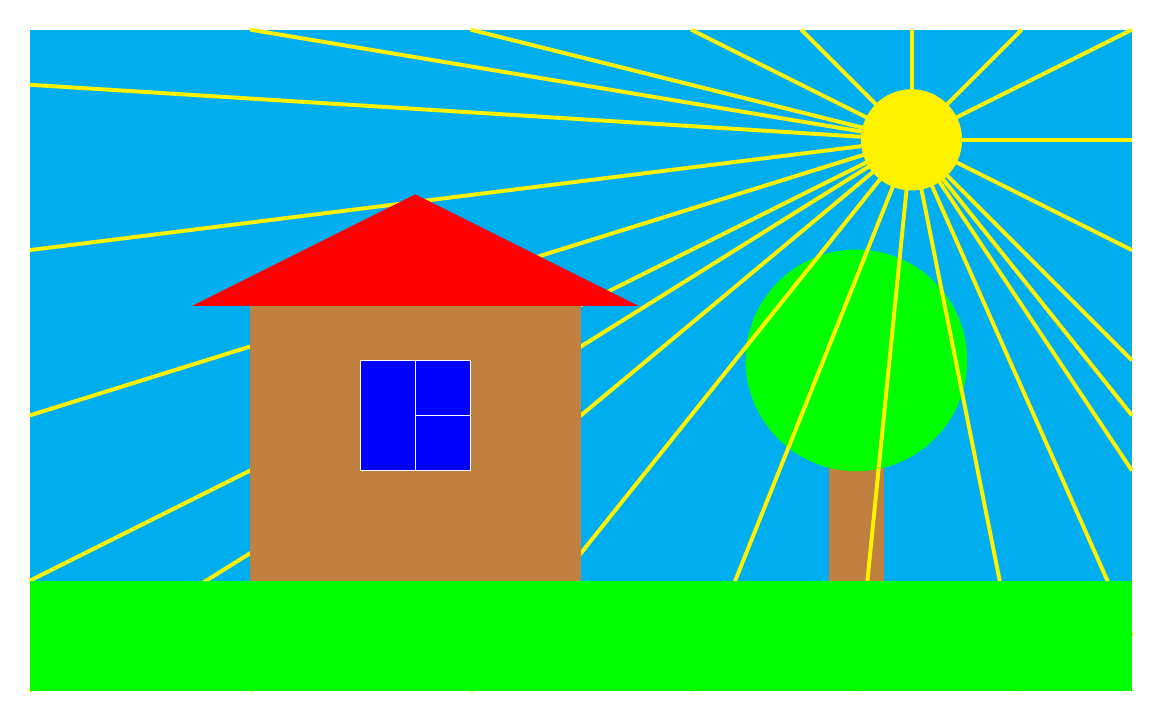
\begin{tikzpicture}[scale=0.7]
\path [draw=none,fill=cyan] (-10,-6) rectangle (10,6);
\path [draw=none,fill=brown] (4.5,-4) rectangle (5.5,0);
\draw[fill=green,green] (5,0) ellipse (20mm and 20mm);
\draw [line width=0.5mm ,yellow] (6,4) to (-10,-6);
\draw [line width=0.5mm ,yellow] (6,4) to (-6,-6);
\draw [line width=0.5mm ,yellow] (6,4) to (-2,-6);
\draw [line width=0.5mm ,yellow] (6,4) to (2,-6);
\draw [line width=0.5mm ,yellow] (6,4) to (5,-6);
\draw [line width=0.5mm ,yellow] (6,4) to (10,-5);
\draw [line width=0.5mm ,yellow] (6,4) to (10,-2);
\draw [line width=0.5mm ,yellow] (6,4) to (8,-6);
\draw [line width=0.5mm ,yellow] (6,4) to (-10,-4);
\draw [line width=0.5mm ,yellow] (6,4) to (-10,-1);
\draw [line width=0.5mm ,yellow] (6,4) to (-10,2);
\draw [line width=0.5mm ,yellow] (6,4) to (-10,5);
\draw [line width=0.5mm ,yellow] (6,4) to (-6,6);
\draw [line width=0.5mm ,yellow] (6,4) to (-2,6);
\draw [line width=0.5mm ,yellow] (6,4) to (2,6);
\draw [line width=0.5mm ,yellow] (6,4) to (4,6);
\draw [line width=0.5mm ,yellow] (6,4) to (6,6);
\draw [line width=0.5mm ,yellow] (6,4) to (8,6);
\draw [line width=0.5mm ,yellow] (6,4) to (10,6);
\draw [line width=0.5mm ,yellow] (6,4) to (10,4);
\draw [line width=0.5mm ,yellow] (6,4) to (10,2);
\draw [line width=0.5mm ,yellow] (6,4) to (10,0);
\draw [line width=0.5mm ,yellow] (6,4) to (10,-1);
\path [draw=none,fill=green] (-10,-4) rectangle (10,-6);
\path [draw=none,fill=brown] (-6,-4) rectangle (-0,1);
\path [draw=none,fill=blue] (-4,-2) rectangle (-2,0);
\draw [- ,white] (-3,-1) to (-2,-1);
\draw [- ,white] (-4,-2) to (-2,-2);
\draw [- ,white] (-4,0) to (-2,0);
\draw [- ,white] (-3,-2) to (-3,0);
\draw [- ,white] (-2,-2) to (-2,0);
\draw [- ,white] (-4,-2) to (-4,0);
\draw [red,fill=red](-7,1) -- (1,1) -- (-3,3) -- cycle;
\draw[fill=yellow,yellow] (6,4) circle (6ex);

\end{tikzpicture}
\end{figure}
\end{document}